\documentclass{report}

\usepackage{titlesec}
\usepackage{tikz}
\usepackage{amsmath}
\usepackage{graphicx}
\usetikzlibrary{arrows}
\graphicspath{ {./images/} }



\titleformat
{\chapter} % command
[display] % shape
{\bfseries\Large\itshape} % format
{} % label (wow, it's **** nothing!)
{0.5ex} % sep
{
    \rule{\textwidth}{1pt}
    \vspace{1ex}
    \centering
} % before-code
[
\vspace{-0.5ex}%
\rule{\textwidth}{0.3pt}
] % after-code


\titleformat{\section}[wrap]
{\normalfont\bfseries}
{\thesection.}{0.5em}{}

\titlespacing{\section}{12pc}{1.5ex plus .1ex minus .2ex}{1pc}

\begin{document}

La aplicacion es un servicio web monolitico de un solo usuario montado sobre django.

El unico usuario, el administrador de la plataforma, maneja los records de la base de datos.
Si hiciera falta crear mas usuarios se puede hacer usando la tabla User default de django y añadiendo dichos usuarios a grupos para asignarle permisos.

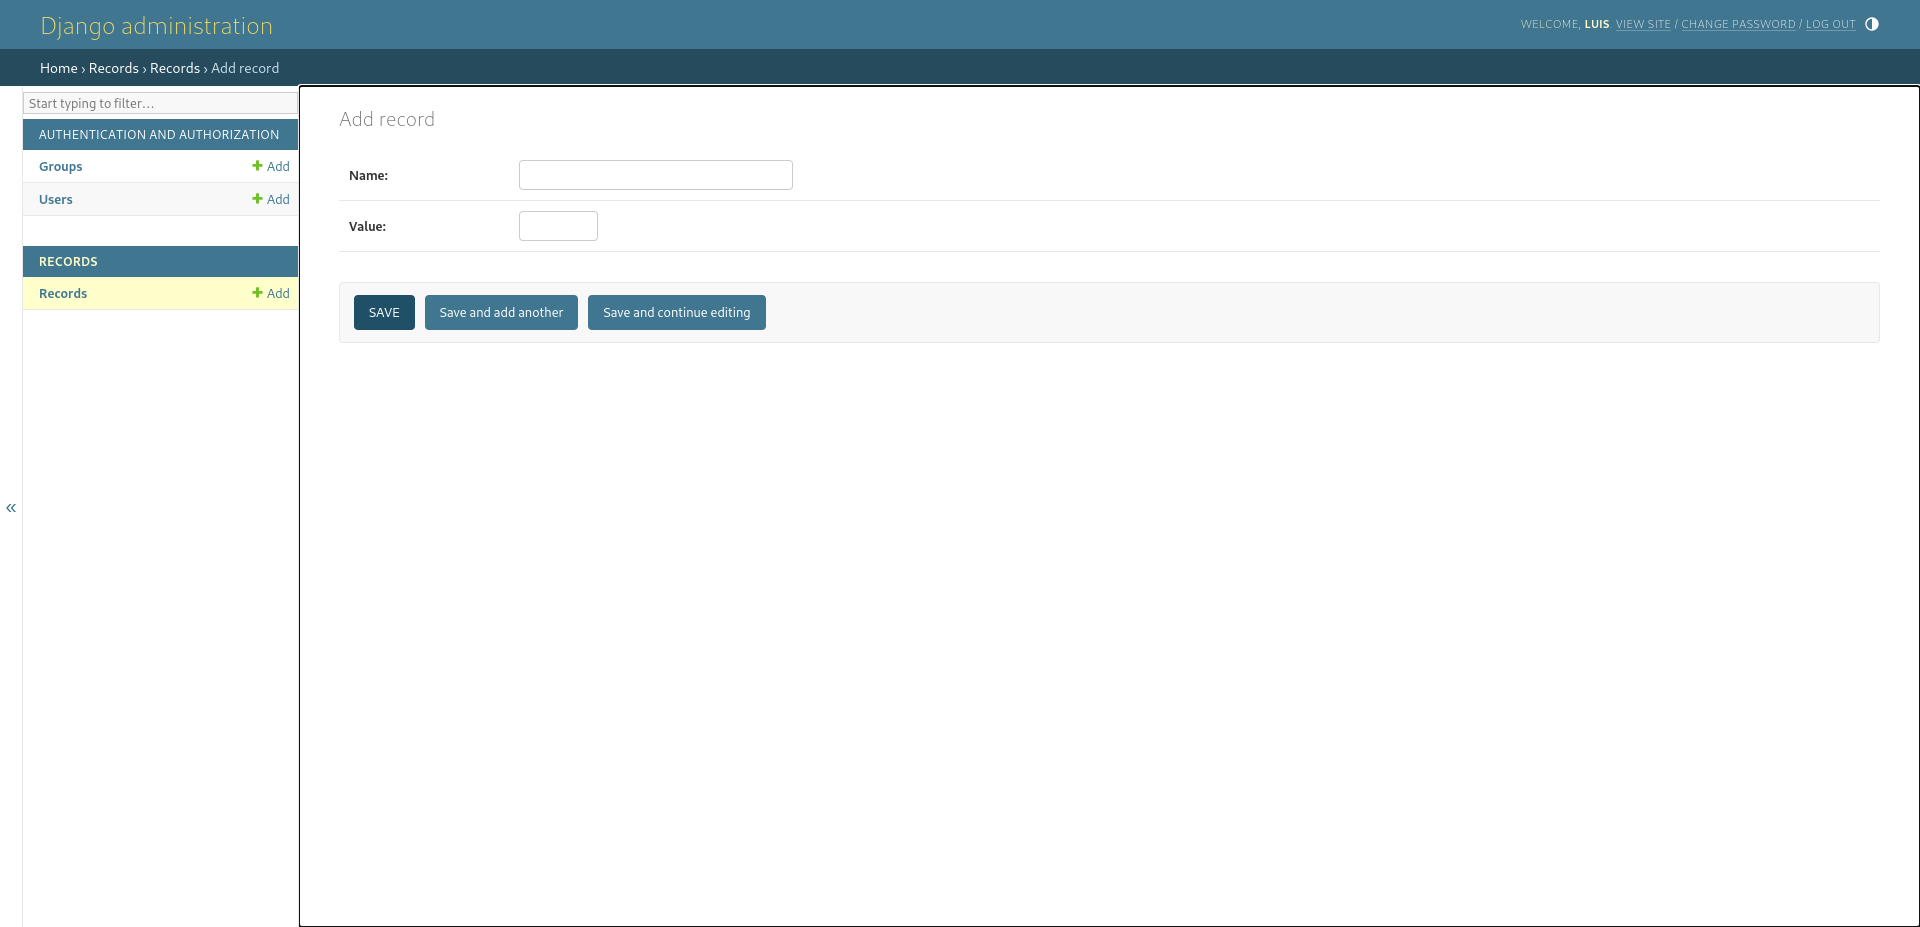
\includegraphics[scale=0.2]{record}

Por ahora la tabla records es un dummy porque no tengo la especificacion de la entrada.
Inclui una API REST con metodos basicos para interactuar con la tabla records (probablemente haga falta mas adelante)

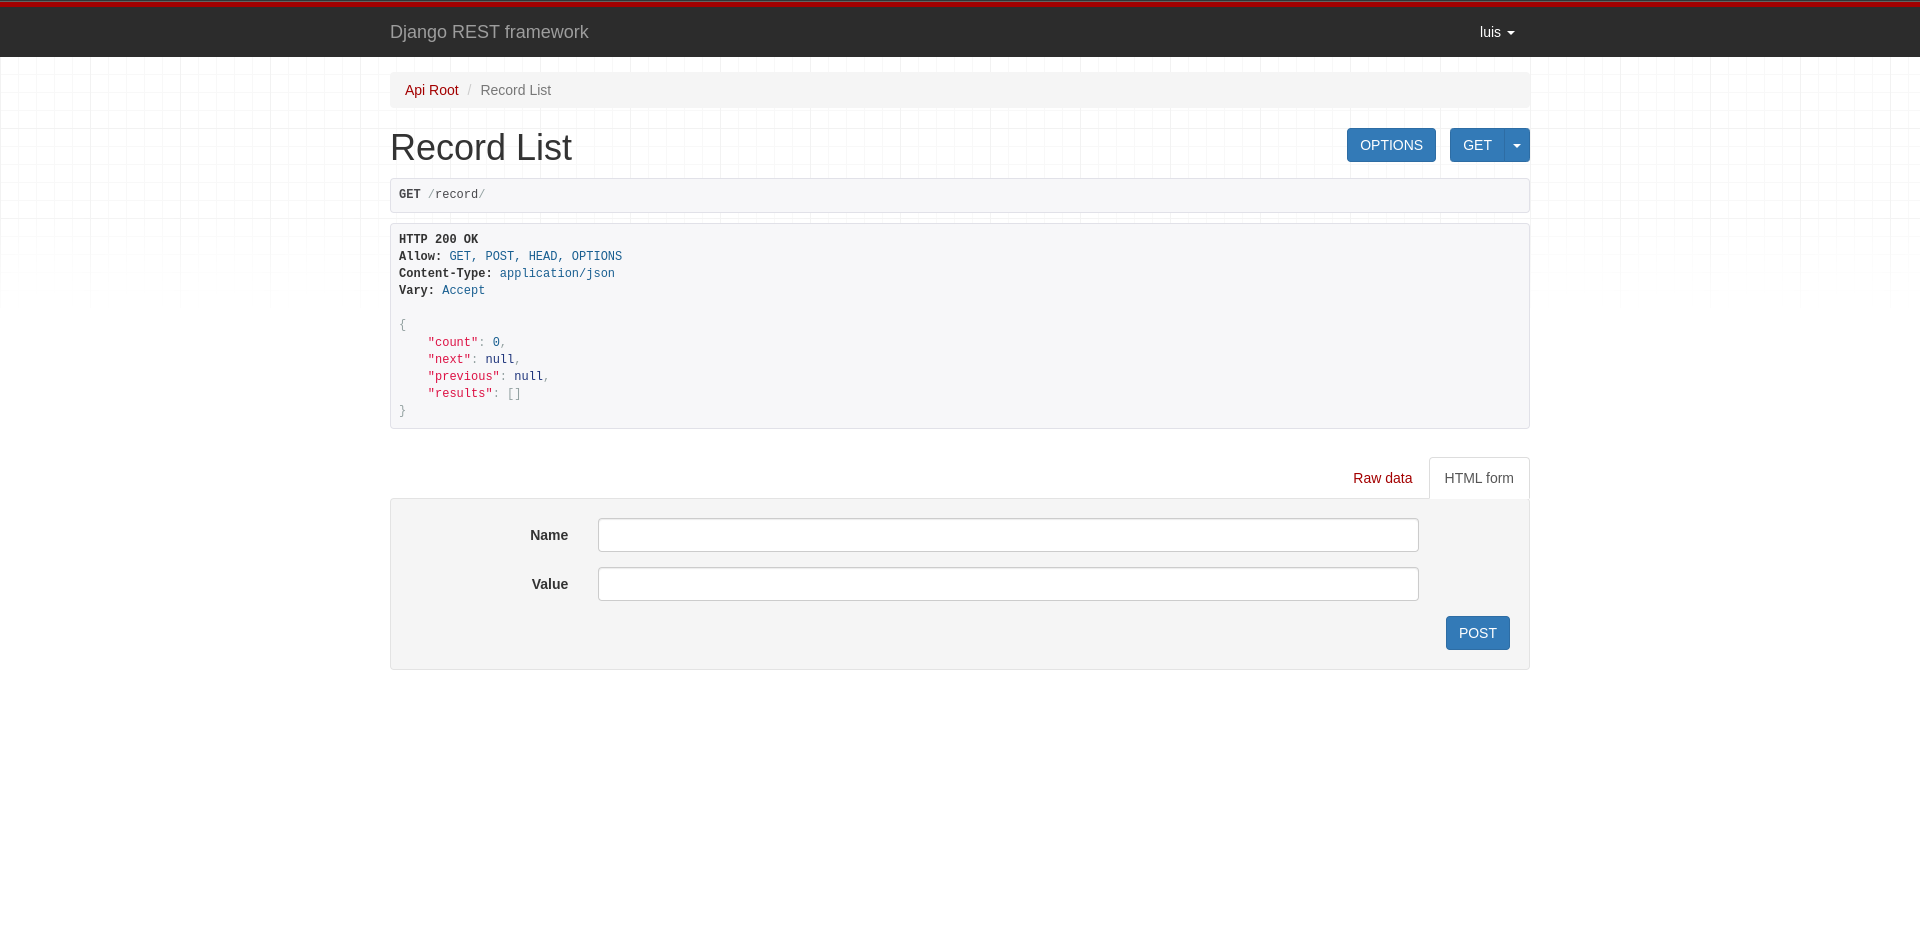
\includegraphics[scale=0.2]{api}

La configuracion de la base de datos es la default. Incluido el campo default de la primary key que django crea para todas las tablas que es un entero de 64 bits autoincrementado.

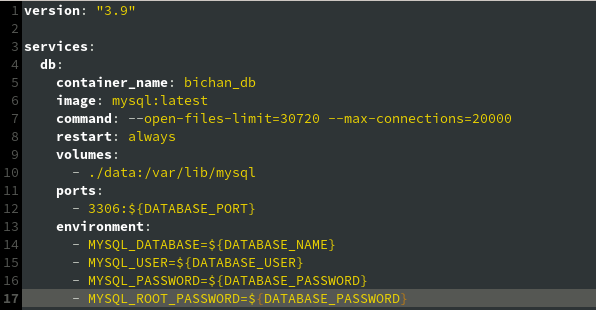
\includegraphics[scale=0.5]{docker}

Los secretos (user, password, nombre de la base de datos) se guardan en un fichero aparte que no se persiste en el control de versiones y en variables de entorno.

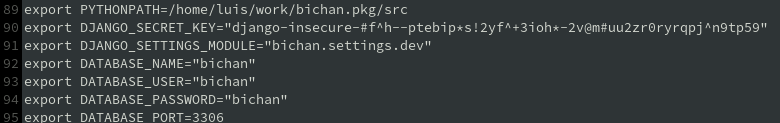
\includegraphics[scale=0.5]{env}
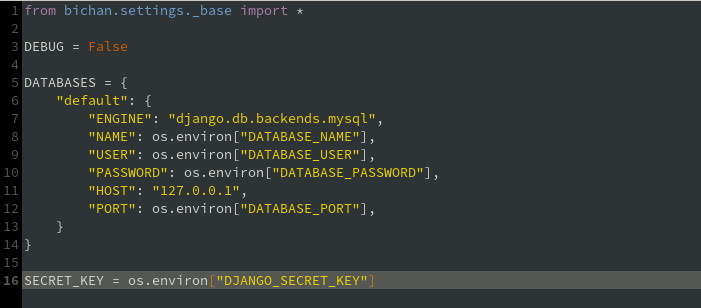
\includegraphics[scale=0.5]{settings}

\end{document}
